\documentclass[twoside]{article}
\usepackage{listings}
\usepackage{color}
\usepackage{verbatim}
\usepackage{amsmath}
\definecolor{dkgreen}{rgb}{0,0.6,0}
\definecolor{gray}{rgb}{0.5,0.5,0.5}
\definecolor{mauve}{rgb}{0.58,0,0.82}
\usepackage{amssymb}
\usepackage{amsthm}
\usepackage{thmtools}
\usepackage{graphicx}


% \lstset{frame=tb,
%   language=Java,
%   aboveskip=3mm,
%   belowskip=3mm,
%   showstringspaces=false,
%   columns=flexible,
%   basicstyle={\small\ttfamily},
%   numbers=none,
%   numberstyle=\tiny\color{gray},
%   keywordstyle=\color{blue},
%   commentstyle=\color{dkgreen},
%   stringstyle=\color{mauve},
%   breaklines=true,
%   breakatwhitespace=true
%   tabsize=3
% }

\lstset{
  aboveskip=0mm,
  belowskip=0mm,
  showstringspaces=false,
  columns=flexible,
  basicstyle={\small\ttfamily},
  numbers=none,
  numberstyle=\tiny\color{gray},
  keywordstyle=\color{blue},
  commentstyle=\color{dkgreen},
  stringstyle=\color{mauve},
  breaklines=true,
  breakatwhitespace=true
  tabsize=3
}

%%%%%%%%%%%%%%%%%%%%%%%%%%%%%%%%%%%%%%%%%
% Stylish Colored Title Page 
% LaTeX Template
% Version 1.0 (27/12/12)
%
% This template has been downloaded from:
% http://www.LaTeXTemplates.com
%
% Original author:
% Peter Wilson (herries.press@earthlink.net)
%
% License:
% CC BY-NC-SA 3.0 (http://creativecommons.org/licenses/by-nc-sa/3.0/)
% 
% Instructions for using this template:
% This title page compiles as is. If you wish to include this title page in 
% another document, you will need to copy everything before 
% \begin{document} into the preamble of your document. The title page is
% then included using \titleBC within your document.
%
%%%%%%%%%%%%%%%%%%%%%%%%%%%%%%%%%%%%%%%%%

%----------------------------------------------------------------------------------------
%	PACKAGES AND OTHER DOCUMENT CONFIGURATIONS
%----------------------------------------------------------------------------------------


\usepackage[svgnames]{xcolor} % Required to specify font color

\newcommand*{\plogo}{\fbox{$\mathcal{PL}$}} % Generic publisher logo


%----------------------------------------------------------------------------------------
%	TITLE PAGE
%----------------------------------------------------------------------------------------

\newcommand*{\rotrt}[1]{\rotatebox{90}{#1}} % Command to rotate right 90 degrees
\newcommand*{\rotlft}[1]{\rotatebox{-90}{#1}} % Command to rotate left 90 degrees
\def \a {NavyBlue}
\def \b {Magenta}
\def \c {Purple}
\def \n {4}
\def \prof {Prof. Prakash Panangaden}
\def \courseTitle {Comp 250}
\def \date {Monday October 20, 2013}
\newcommand*{\titleBC}[4]{\begingroup % Create the command for including the title page in the document
\centering % Center all text

\def\CP{\textit{\Huge Assignment #1}} % Title

%\settowidth{\unitlength}{\CP} % Set the width of the curly brackets to the width of the title
%{\color{LightGoldenrod}\resizebox*{\unitlength}{\baselineskip}{\rotrt{$\}$}}} \\[\baselineskip] % Print top curly bracket
%\textcolor{Sienna}{\CP} \\[\baselineskip] % Print title
%{\color{RosyBrown}\Large for Prof. Sergey Norin} \\ % Tagline or further description
%{\color{LightGoldenrod}\resizebox*{\unitlength}{\baselineskip}{\rotlft{$\}$}}} % Print bottom curly bracket


\settowidth{\unitlength}{\CP} % Set the width of the curly brackets to the width of the title
{\color{\a}\resizebox*{\unitlength}{\baselineskip}{\rotrt{$\}$}}} \\[\baselineskip] % Print top curly bracket
\textcolor{\b}{\CP} {\color{\a}{\\ #2}} \\[\baselineskip] % Print title
{\color{\c}\Large for #3} \\ % Tagline or further description
{\color{\a}\resizebox*{\unitlength}{\baselineskip}{\rotlft{$\}$}}} % Print bottom curly bracket

%Default are LightGoldenrod / Sienna / RosyBrown / LightGoldenrod

%\vfill % Whitespace between the title and the author name
\vspace*{\fill}
{\Large\textbf{by Alan Do-Omri\\260532985}}\\ % Author name
\vspace*{\fill}
#4

\endgroup}
\linespread{1.05}
\usepackage{lipsum}
\usepackage{multicol}
\usepackage{alltt}
\usepackage[margin=1in]{geometry}
\usepackage{mathtools}
% \usepackage{subcaption}
\usepackage{hyperref}
\usepackage{paralist}
\usepackage{float}
\usepackage{microtype}
\usepackage{abstract}
\usepackage[utf8]{inputenc}
\usepackage[numbers]{natbib}
\usepackage{graphicx}
\renewcommand{\abstractnamefont}{\large\bfseries} % Set the "Abstract" text to bold
\renewcommand{\abstracttextfont}{\normalfont\itshape} % Set the abstract itself to small italic text
\usepackage{lettrine}
\usepackage{tabulary}
\usepackage{import}
\usepackage{enumitem}
\usepackage{pgf}
\usepackage{caption}
\newenvironment{Figure}
  {\par\medskip\noindent\minipage{\linewidth}}
  {\endminipage\par\medskip}

\usepackage{titlesec} % Allows customization of titles
%\renewcommand\thesection{\Roman{section}} % Roman numerals for the sections
%\renewcommand\thesubsection{\Roman{subsection}} % Roman numerals for subsections
\titleformat{\section}[block]{\Large\scshape\centering\bfseries}{\thesection.}{1em}{} % Change the look of the section titles
\titleformat{\subsection}[block]{\large\bfseries}{\thesubsection.}{1em}{} % Change the look of the section titles

\usepackage{fancyhdr} % Headers and footers
\pagestyle{fancy} % All pages have headers and footers
\fancyhead{} % Blank out the default header
\fancyfoot{} % Blank out the default footer
\fancyhead[C]{Virus Classification from Transmission Electron Microscopy $\bullet$ Fall 2015} % Custom header text
\fancyfoot[RO,LE]{\thepage} % Custom footer text

\title{\fontsize{18pt}{10pt}\textbf{Classifiying Transmission Electron Microscopy Virus Textures}} % Article title

% \author{
% \large{Alan Do-Omri}\\[2mm] % Your name
% \normalsize McGill University \\ % Your institution
% \normalsize \href{mailto:alan.do-omri@mail.mcgill.ca}{alan.do-omri@mail.mcgill.ca}}

\author{
\large{Alan Do-Omri}\\[2mm] 
\normalsize 260532985 \\ 
\and 
\large{Kian Kenyon-Dean}\\[2mm]
\normalsize 260564475 \\
\and
\large{Genevieve Fried}\\[2mm]
\normalsize 260564432 \\
}


\begin{document}

\maketitle

\begin{abstract}
Determining the identity of a virus sample is of utmost importance in today's medical community. An incorrect classification of the virus can be life-threatening not only to the patient, but to people surrounding him or her. A transmission electron microscopy image of a virus sample can be hard to discern for the human eye and a doctor needs to be positive about the identity of the virus i.e., if it's Influenza or Ebola. Fortunately, machine learning algorithms perform exceedingly well on image classification tasks and don't require expert knowledge to do so. Here we present a successful application of using convolutional neural networks to classify viruses samples into one of 15 categories and compare its performance to previous work done on the same task.
\end{abstract} 
\vspace{0.5cm}

\begin{multicols}{2}
\section{Introduction}
\section{Related Work}
In the work of \citet{kylberg2011virus}, texture analysis is performed on the virus samples and the resulting feature vector is fed to a Random Forest classifier. They are comparing the performance of different texture analysers such as Local Binary Patterns and Radial Density Profile along with their respective variants. First, we will briefly explain the feature extractors they used. Then, we will present the results they got. 
\subsection{Local Binary Profile (LBP)}
Given an image, for each pixel $p_i$ in it, sample $n$ equally-spaced points on the circle of radius $r$ with center $p_i$ -- an example of sampling is shown in figure \ref{fig:lbp_basic} -- and construct a vector $v(p_i)$ such that its $i$th entry is a 1 if the $i$th sampled pixel has a value bigger than $p_i$ or a 0 otherwise. 
\begin{figure*}
	\centering
	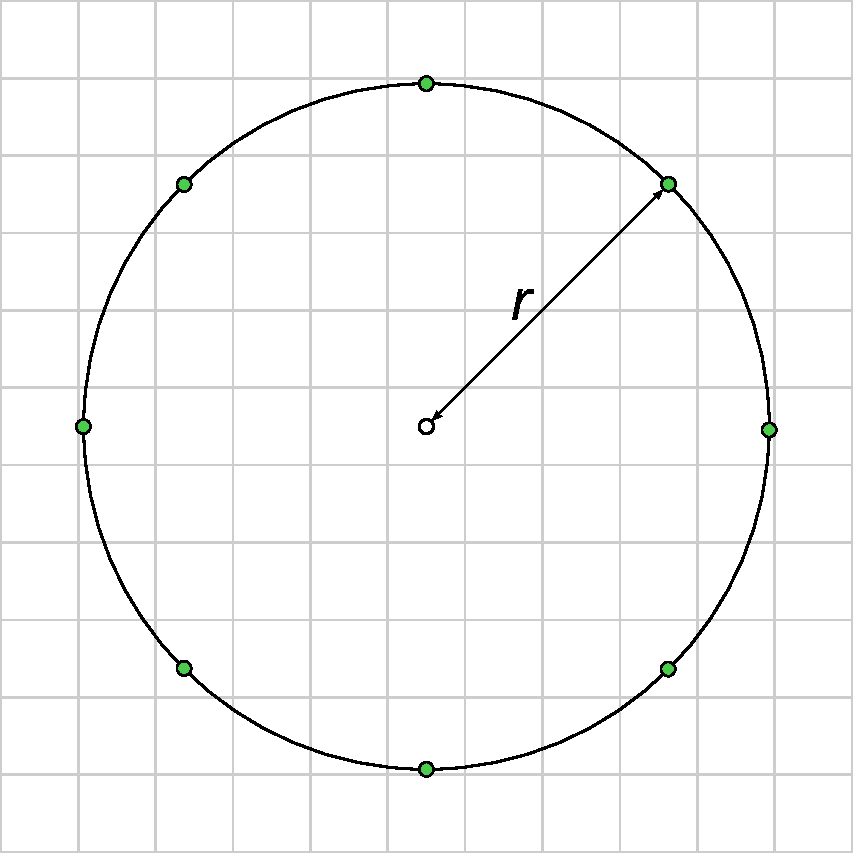
\includegraphics[width=0.5\linewidth]{images/lbp_basic.pdf}
	\captionof{figure}{Example of LBP sampling: The green points are the neighbouring sample points at distance $r$ from the central white point. In this case, we are sampling with $n=8$ neighbour points.}
	\label{fig:lbp_basic}
\end{figure*}
With its sequence of 0s and 1s, $v(p_i)$ now makes a binary number $v_{p_i}$, hence the name. Once we have the $v_{p_i}$ for all pixels, we construct a histogram counting the number of appearances of each value $v_{p_i}$. The histogram is the feature vector associated with the given image. \citet{kylberg2011virus} denote this feature extraction method by LBP$_{n, r}$, where $n$ is the number of sampled points and $r$ is the radius, as described above. The resulting histogram is represented in a vector of counts with $2^n$ elements. 
\paragraph{Rotational Invariant LBP} In order to reduce the size of that feature vector, \citet{kylberg2011virus} mention a modification of LBP in the following sense: instead of creating $v_{p_i}$ by interpreting the vector $v(p_i)$ and using $v_{p_i}$ as is, rotate the number $v_{p_i}$ bitwise until you get the smallest possible number. For example, the number 110 would turn into 011. They name it rotational invariant and denote it with LBP$^{\textnormal{ri}}_{n,r}$.
\paragraph{Uniform LBP} To further reduce the size of the histogram, they also try restricting the values of $v_{p_i}$ to only numbers that have 2 or less transitions from 0 to 1 or from 1 to 0 and they call this variant \emph{uniform binary patterns with at most 2 spatial transitions}, denoted LBP$^{\textnormal{u2}}_{n,r}$. For example, 01010 has 2 transitions from 0 to 1 and 2 transitions from 1 to 0 which makes 4 transitions in total so this version LBP$^{\textnormal{u2}}_{n,r}$ would not count that number. On the other hand, 00111 has only 1 transition from 0 to 1 so it is accepted. 
\par 
\paragraph{Gaussian Filtered LBP} Finally, \citet{maenpaa2003multi} talk about an extension to the LBP that is also used in the work of \citet{kylberg2011virus} which consists in sampling the neighbours at different radii around the central pixel. Additionally, instead of sampling on circles with points spread in an equi-distant fashion, they would be sampled according to a Gaussian distribution. Figure \ref{fig:rdp} shows an example of such a sampling. \citet{kylberg2011virus} denote it as LBPF$^{\textnormal{ri}}_{n_1,r_1}$ $+$ $^{\textnormal{ri}}_{n_2,r_2}$ $+$ $\cdots$ $+$ $^{\textnormal{ri}}_{n_j,r_j}$ for the different numbers of sample points $n_1, n_2, \cdots, n_j$ and different radii distances $r_1, r_2, \cdots, r_j$.
\begin{figure*}
	\centering
	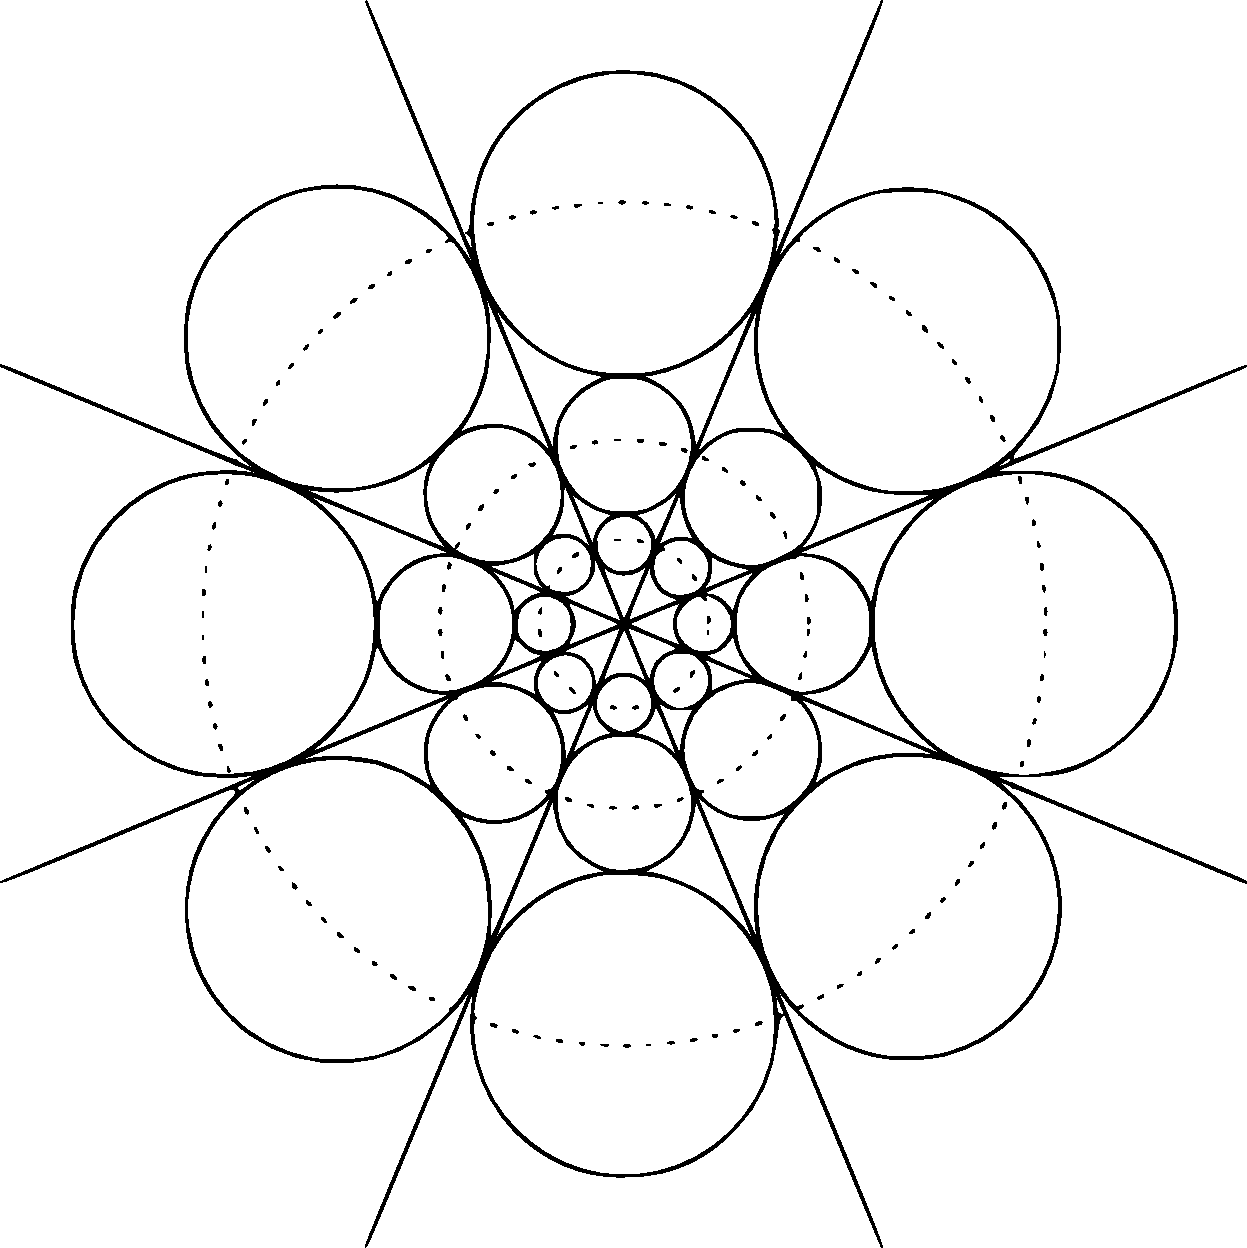
\includegraphics[width=0.5\linewidth]{images/lbpf.pdf}
	\captionof{figure}{Example of LBPF sampling: In the simple LBP, the points would be sampled at equal distances around the dotted circles for one radius as in figure \ref{fig:lbp_basic} but with this extension, the points are sampled according to a Gaussian distribution inside the solid black circles at multiple radii. In this picture, the number of neighbours also vary with the radii. This image comes from \citet{maenpaa2003multi}.}
	\label{fig:lbpf}
\end{figure*}
\subsection{Radial Density Profile (RDP)}
This method is a way to get the mean intensity in a ring around each pixel in the image. \citet{kylberg2011virus} defines the \emph{radial mean intensity $f$} around a center pixel $q_c$ as 
\[ f(q_c, r) = \frac{1}{|N|} \sum\limits_{q\in N} I(q) \]
where $I(q)$ is the pixel value for pixel $q$ and $N = \left\{ q: \Vert q-q_c \Vert_2 \in \left( r-\frac{1}{2}, r+\frac{1}{2} \right] \right\}$ is the set of pixels in a ring around $q_c$ of width 1 at distance $r$ from $q_c$. Figure \ref{fig:rdp} shows an example of what the set $N$ may look like. Following the notation from \citet{kylberg2011virus}, let $\bar{f}_{q_c}$ be the mean of the set $\{ f(q_c,i) \}_{i = 1, \cdots, n}$. Then they define the radial density profile for that pixel $q_c$ as $\textnormal{RDP}_n = \left[ f(q_c,1)-\bar{f}_{q_c}, f(q_c, 2)-\bar{f}_{q_c}, \cdots, f(q_c,n)-\bar{f}_{q_c} \right]$. 
\begin{figure*}
	\centering
	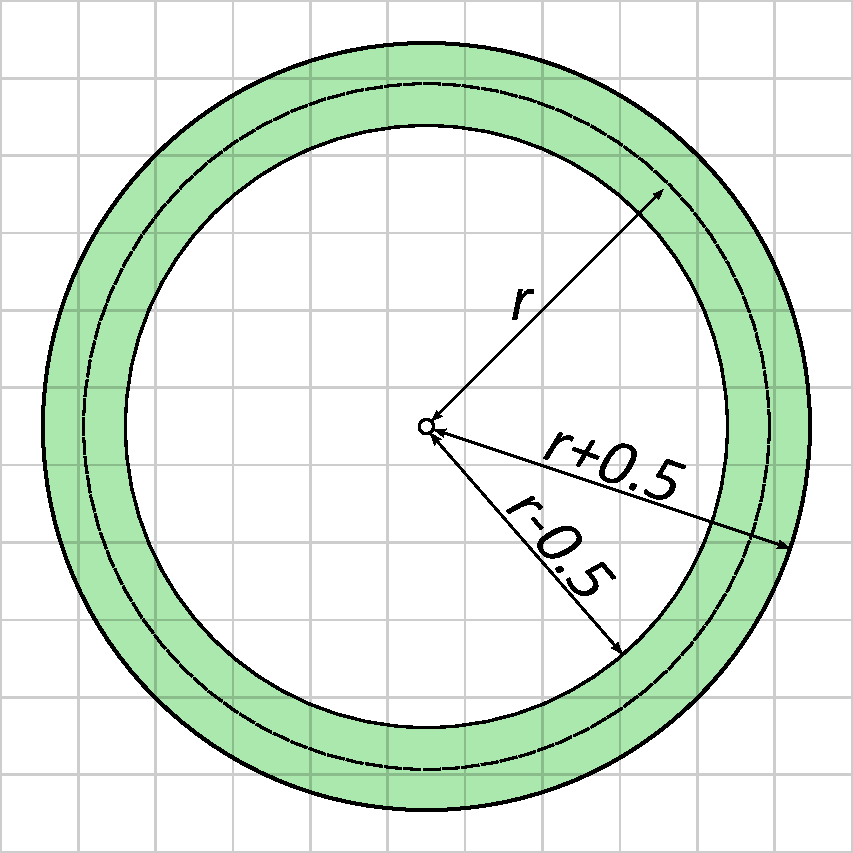
\includegraphics[width=0.5\linewidth]{images/rdp.pdf}
	\captionof{figure}{Example of RDP sampling: The green zone is the set of sampled pixels for a given radius $r$.}
	\label{fig:rdp}
\end{figure*}
\par It is not explained how the pixel features are combined to make the feature vector for the whole image but we would imagine that the feature vector for the whole image is either a concatenation of the pixel features or the concatenation of the mean of each pixel feature. 
\paragraph{Fourier RDP} One variation \citet{kylberg2011virus} introduced is applying the same RDP technique on the image after it undergoes a Fourier transform and looking at it with respect to a base $e$ logarithmic scale. They denote it with FRDP$_n$. 

\newpage
\bibliography{ref}
\bibliographystyle{plainnat}
\end{multicols}
\end{document}
